\section{Genre Game dan Karakteristiknya}

\begin{learningoutcomes}
\item Mengidentifikasi berbagai genre game utama
\item Menjelaskan karakteristik setiap genre
\item Menganalisis mekanik khas dari setiap genre
\item Menerapkan pengetahuan genre dalam desain game
\end{learningoutcomes}

\subsection{Pengertian Genre Game}

\begin{definisi}[Genre Game]
Genre game adalah kategori yang mengklasifikasikan game berdasarkan mekanik gameplay, setting, atau gaya permainan yang dominan \cite{Schell2019}.
\end{definisi}

Genre membantu pemain memahami apa yang diharapkan dari sebuah game dan membantu developer mengkomunikasikan konsep game mereka.

\subsection{Genre Game Utama}

\begin{figure}[ht]
    \centering
    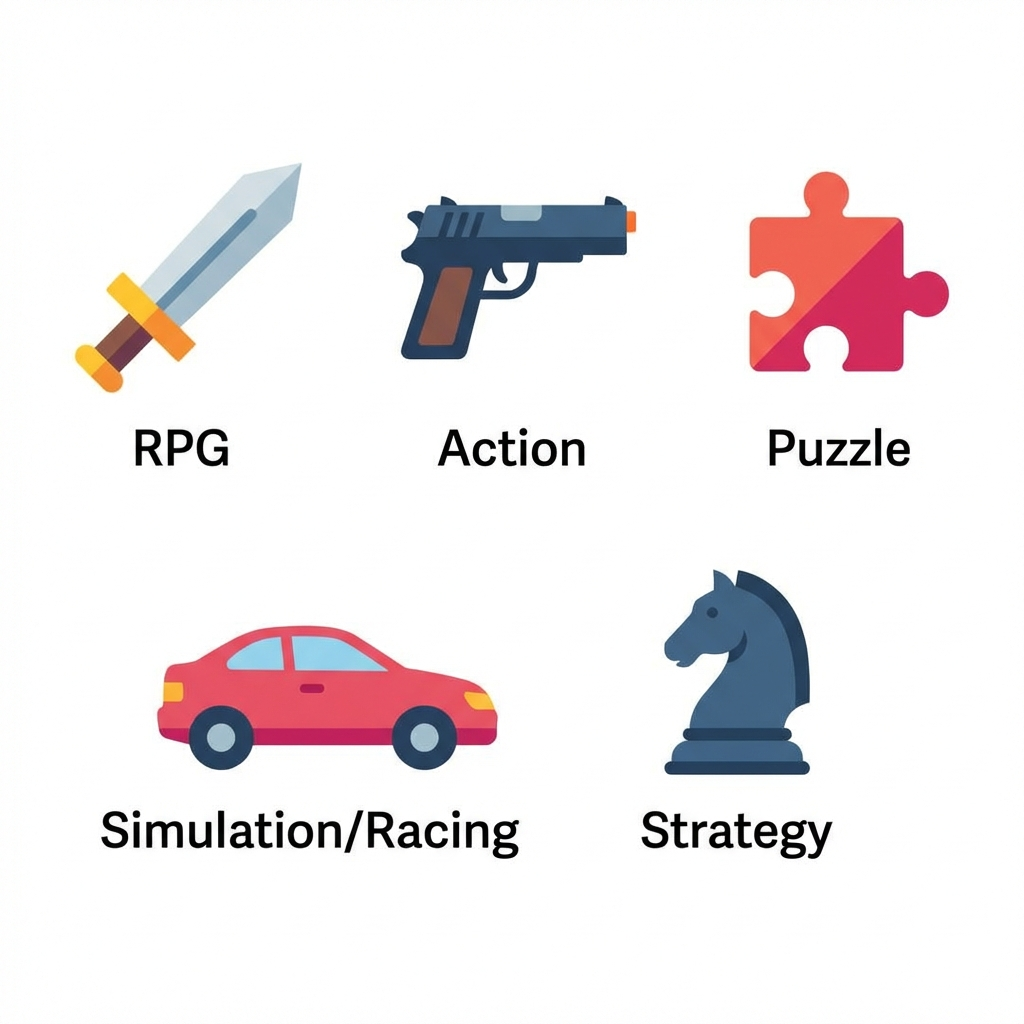
\includegraphics[width=0.8\textwidth]{figures/game_genres.png}
    \caption{Visualisasi Ikon Genre Game Utama}
    \label{fig:game_genres}
\end{figure}

\subsubsection{Action Games}

\textbf{Karakteristik}: Fokus pada refleks dan koordinasi tangan-mata, gameplay cepat dan intens, sering melibatkan combat atau konflik langsung. Contoh: Call of Duty, Devil May Cry, Dark Souls.

\textbf{Sub-genre}: First-Person Shooter (FPS), Third-Person Shooter (TPS), Hack and Slash, Beat 'em up

\subsubsection{Adventure Games}

\textbf{Karakteristik}: Fokus pada narasi dan eksplorasi, puzzle-solving sebagai mekanik utama, interaksi dengan karakter dan lingkungan. Contoh: The Legend of Zelda, Uncharted, Life is Strange.

\subsubsection{Role-Playing Games (RPG)}

\textbf{Karakteristik}: Karakter development dan progression, sistem statistik (HP, MP, Level), quest dan mission-based gameplay. Contoh: Final Fantasy, The Elder Scrolls, The Witcher.

\subsubsection{Strategy Games}

\textbf{Karakteristik}: Fokus pada perencanaan dan taktik, resource management, decision-making jangka panjang. Contoh: Civilization, StarCraft, XCOM.

\subsubsection{Simulation Games}

\textbf{Karakteristik}: Simulasi sistem kehidupan nyata, realisme dan akurasi, open-ended gameplay. Contoh: The Sims, SimCity, Flight Simulator.

\subsubsection{Sports Games}

\textbf{Karakteristik}: Simulasi olahraga nyata, realisme dalam gameplay, multiplayer competitive. Contoh: FIFA, NBA 2K.

\subsubsection{Puzzle Games}

\textbf{Karakteristik}: Fokus pada problem-solving, logic-based challenges, sering tidak memiliki time pressure. Contoh: Tetris, Portal, The Witness.

\subsubsection{Platformer Games}

\textbf{Karakteristik}: Fokus pada jumping dan navigation, level design dengan platform, precision movement. Contoh: Super Mario Bros, Celeste, Hollow Knight.

\subsection{Hybrid Genre}

Banyak game modern menggabungkan elemen dari beberapa genre: Action-RPG, Survival Horror, Metroidvania.

\begin{catatan}
Genre bukanlah kategori yang kaku. Game modern sering menggabungkan elemen dari berbagai genre untuk menciptakan pengalaman yang unik.
\end{catatan}
